\question[3]
Der Graph wird von Startknoten a aus mit Tiefensuche traversiert. Die
  Nachbarn werden in alphabetischer Reihenfolge besucht.
  Schreibe an die Knoten ihre previsit/postvisit Nummern.

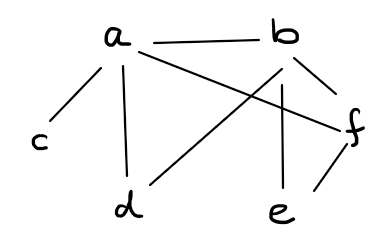
\includegraphics[height=4cm]{\pfad/Graphen/Aufgaben/visit_03/visit_03.png}

\ifprintanswers
Lösung:
\begin{lstlisting}
a  1 12
b  2  9
d  3  4
e  5  8
f  6  7
c  10 11
\end{lstlisting}
\fi
